\documentclass[a4j,uplatex, fleqn]{jsarticle} % [A4 uplatex 数式を左寄せに]{和文の論文}

% =========使用パッケージの宣言=========
% 画像関係のパッケージ
\usepackage[dvipdfmx]{graphicx}
\usepackage[dvipdfmx]{color}
% 数式関係
\usepackage{siunitx}
\usepackage{amsmath}
\usepackage{amssymb}
% 表でHを使う
\usepackage{float}
% セルに斜線を入れる
\usepackage{diagbox}
% セル結合を使えるようにする
\usepackage{booktabs, multirow}
% 複数ページに渡る表を作る
\usepackage{longtable}
% 参考文献用,URLの埋め込み用
\usepackage{url}

% =========カスタム設定=========
% 数式番号を(セクション番号.式番号)の形式にする e.g. (2.1)
\numberwithin{equation}{section}
% bulletより小さい丸,sbt
\newcommand{\sbt}{\,\begin{picture}(-1,1)(-1,-3)\circle*{3}\end{picture}\ }

% =========タイトル・作成者・日付の設定=========
\title{\LaTeX でレポートを作成するサンプル文章}
\author{だつかくあーてぃー}
\date{}

\begin{document}
	% タイトルと作成者、作成日の記入編
	\maketitle

	% 見出し編
	\section{ここは第1節の見出しになります}
		ここは第1節の本文になります。
		\subsection{ここは第1小節の見出しになります}
			ここは第1小節の本文になります。
			\subsubsection{ここは第1小小節の見出しになります}
				ここは第1小小節の本文になります。
				\paragraph{ここは第1段落の見出しになります}
					ここは第1段落の本文になります。
	\section*{この節には、番号が振られません}
		ここの節は付録とかに使ってください
	
	% 数式編
	\section{数式編} \label{math_mode}
		\subsection{各行に番号振り分け}
			各行ごとに式番号を割り振る場合は$align$環境で行います。
			\begin{align}
				F &= G \frac{Mm}{r^{2}} \\
				G &= F \frac{r^2}{Mm} \label{eq:univ_gravity} \\
				& \mbox{これは万有引力の方程式です。}
			\end{align}
			式\ref{eq:univ_gravity}は万有引力の方程式を示しています。
		\subsection{各行に番号を振り分けない}
			\begin{align*}
				\frac{Z_0}{j tan \beta l} &= j \omega L \\
				- \frac{Z_0}{tan \beta l} &= \omega L \\
				\mbox{$\omega = 2 \pi f なので$} \\
				- \frac{Z_0}{tan \beta l} &= 2 \pi f L \\
				-tan \beta l &= \frac{50}{2 \pi \times 2.45 \times 10^9 \times 15 \times 10^9} \\
				- \beta l &= 12.2\cdots \\
				\therefore \beta l &= 167.8[deg] \stepcounter{equation}\tag{\theequation} \label{eq:inductor}
			\end{align*}
			\mbox{\\stepcounter\{equation\}\\tag\{\\theequation\}}を使うことで式\ref{eq:inductor}のみ、式番号が付与されます。
		\subsection{インラインで数式を書きたい}
			ドルマークでかこむことで、$S(A)+\int_{X}^{} \frac{d^{\prime}Q}{T_e} \leq S(B)$のように文章の途中で数式をかけます。
	% 画像編
	\section{画像編}
		\begin{figure}[H]
			\centering
			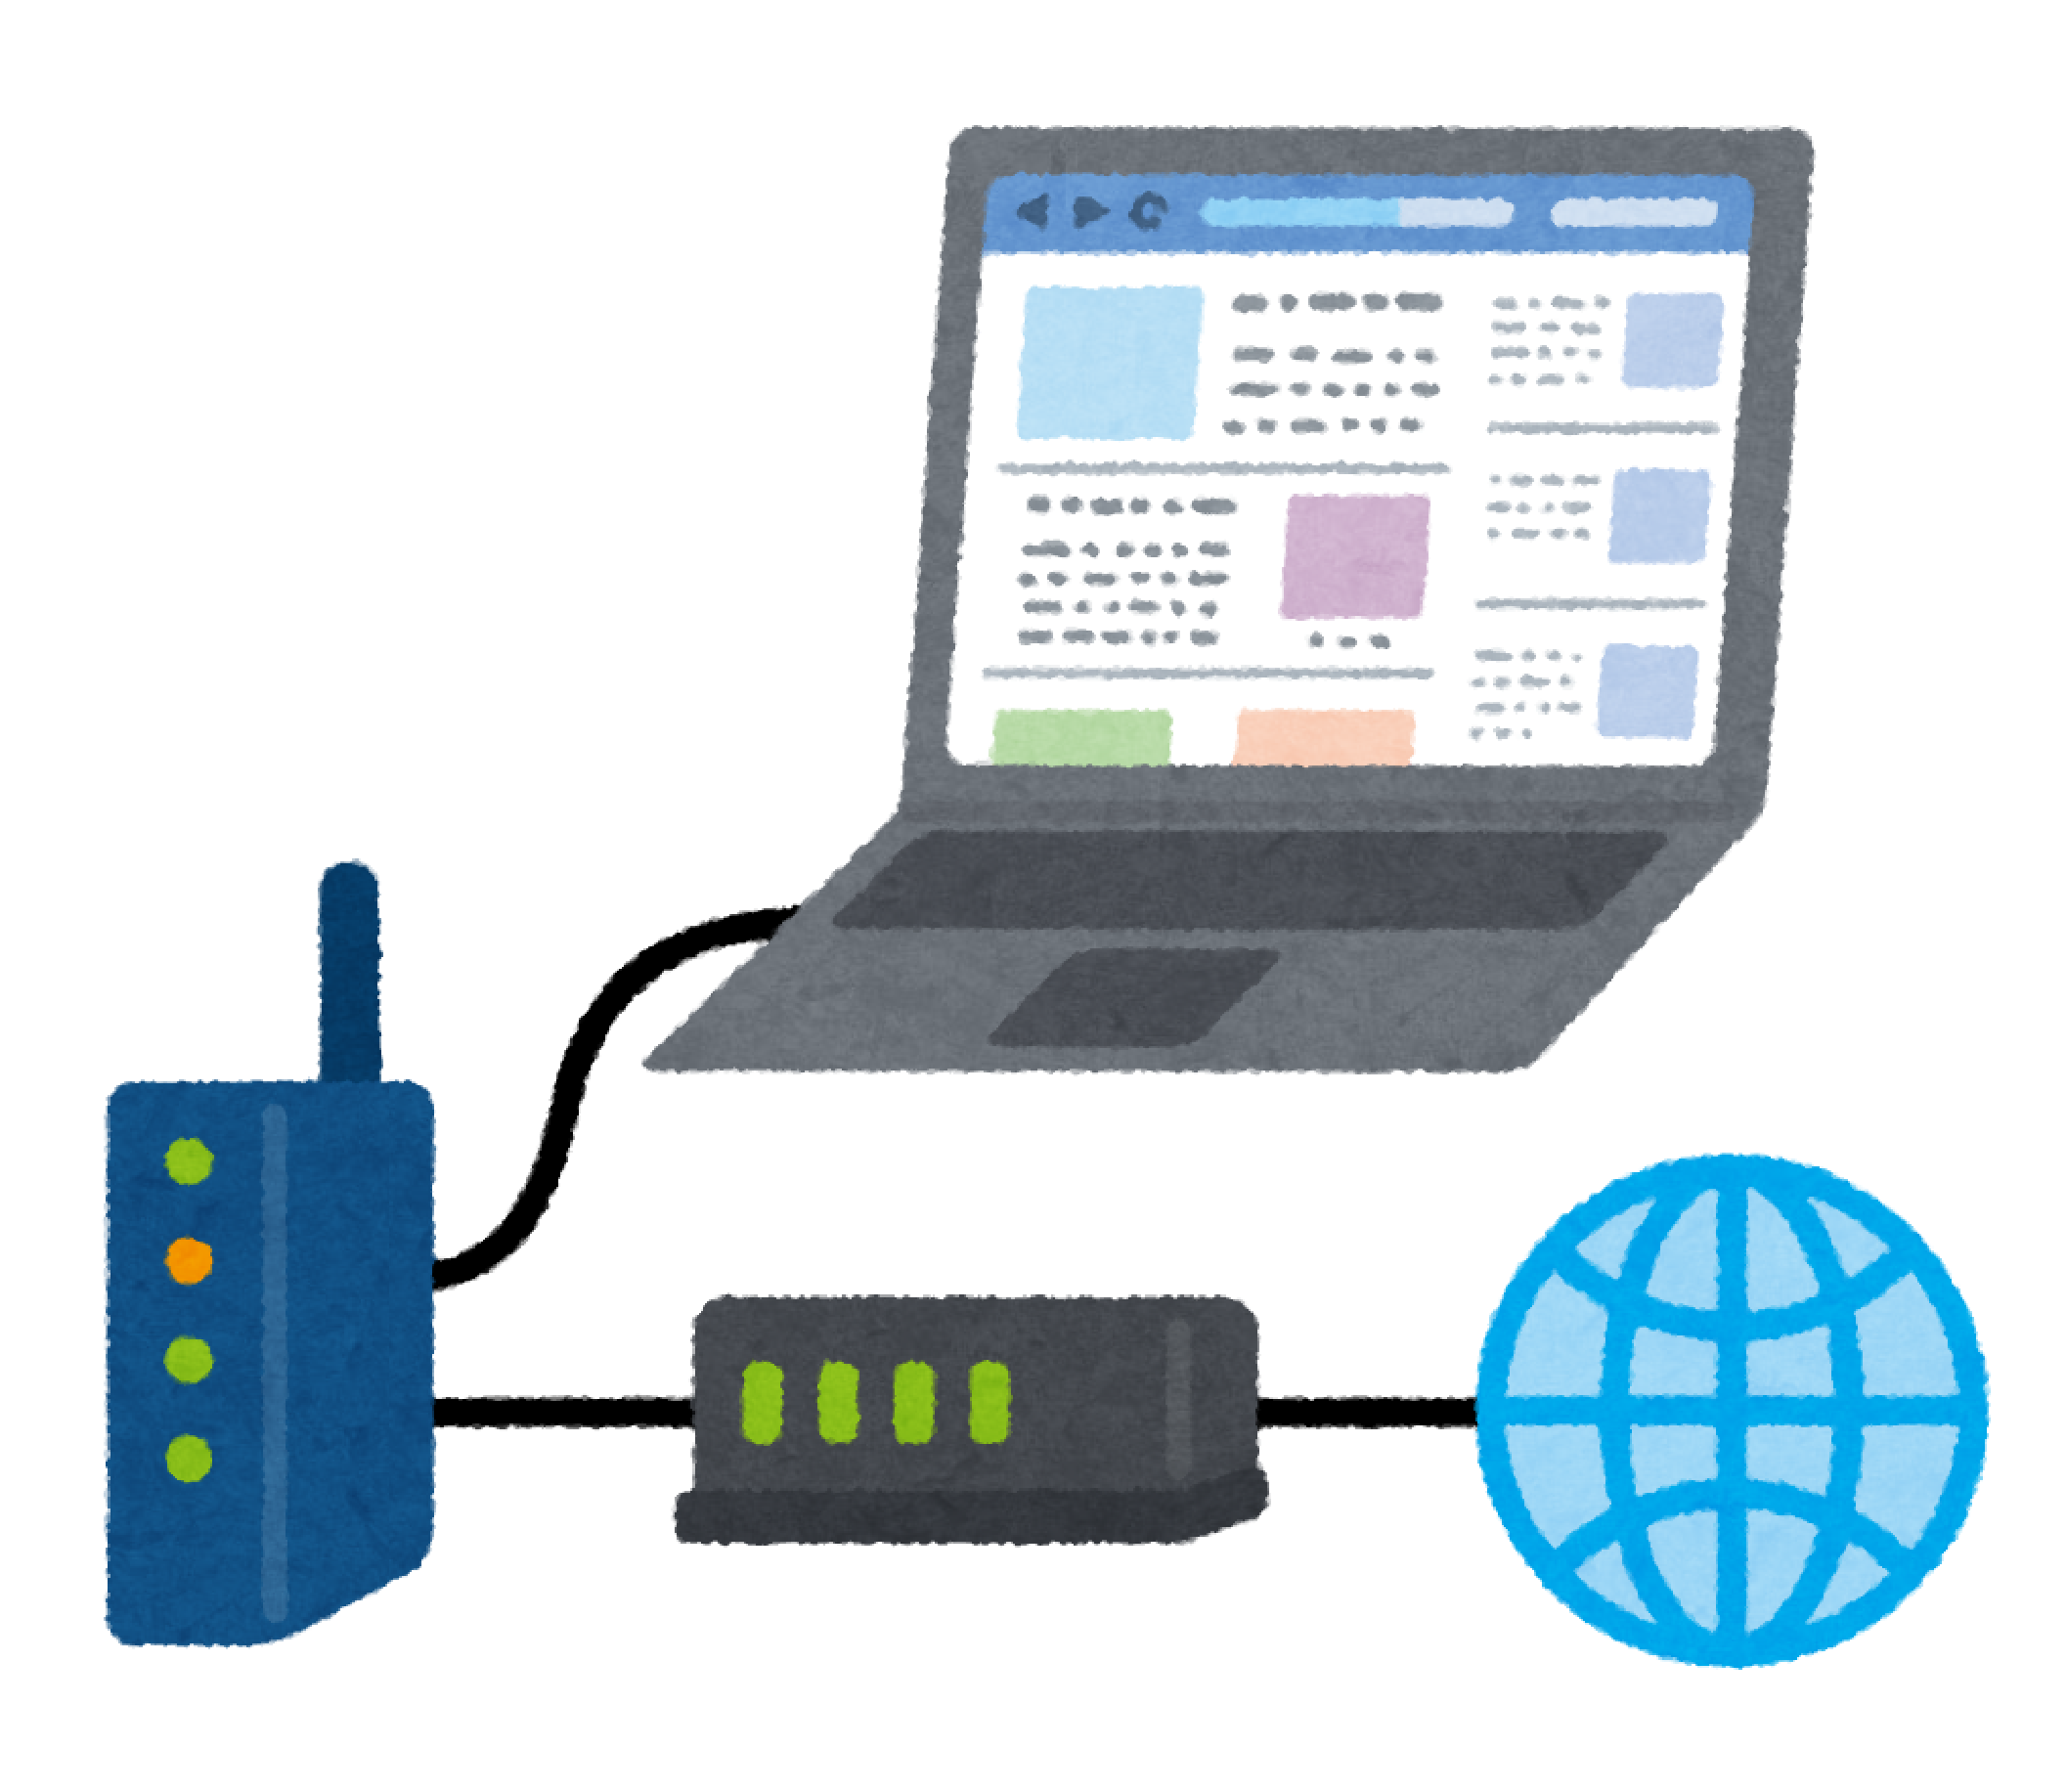
\includegraphics[width=14cm]{./pic/internet_computer_wired.png.pdf}
			\caption{いらすとや・有線LAN接続のいらすと \label{fig:wired_no1}}
		\end{figure}
		\subsection{画像を並べる}
			\begin{figure}[H]
				\begin{minipage}[c]{0.5\hsize}
				\centering
				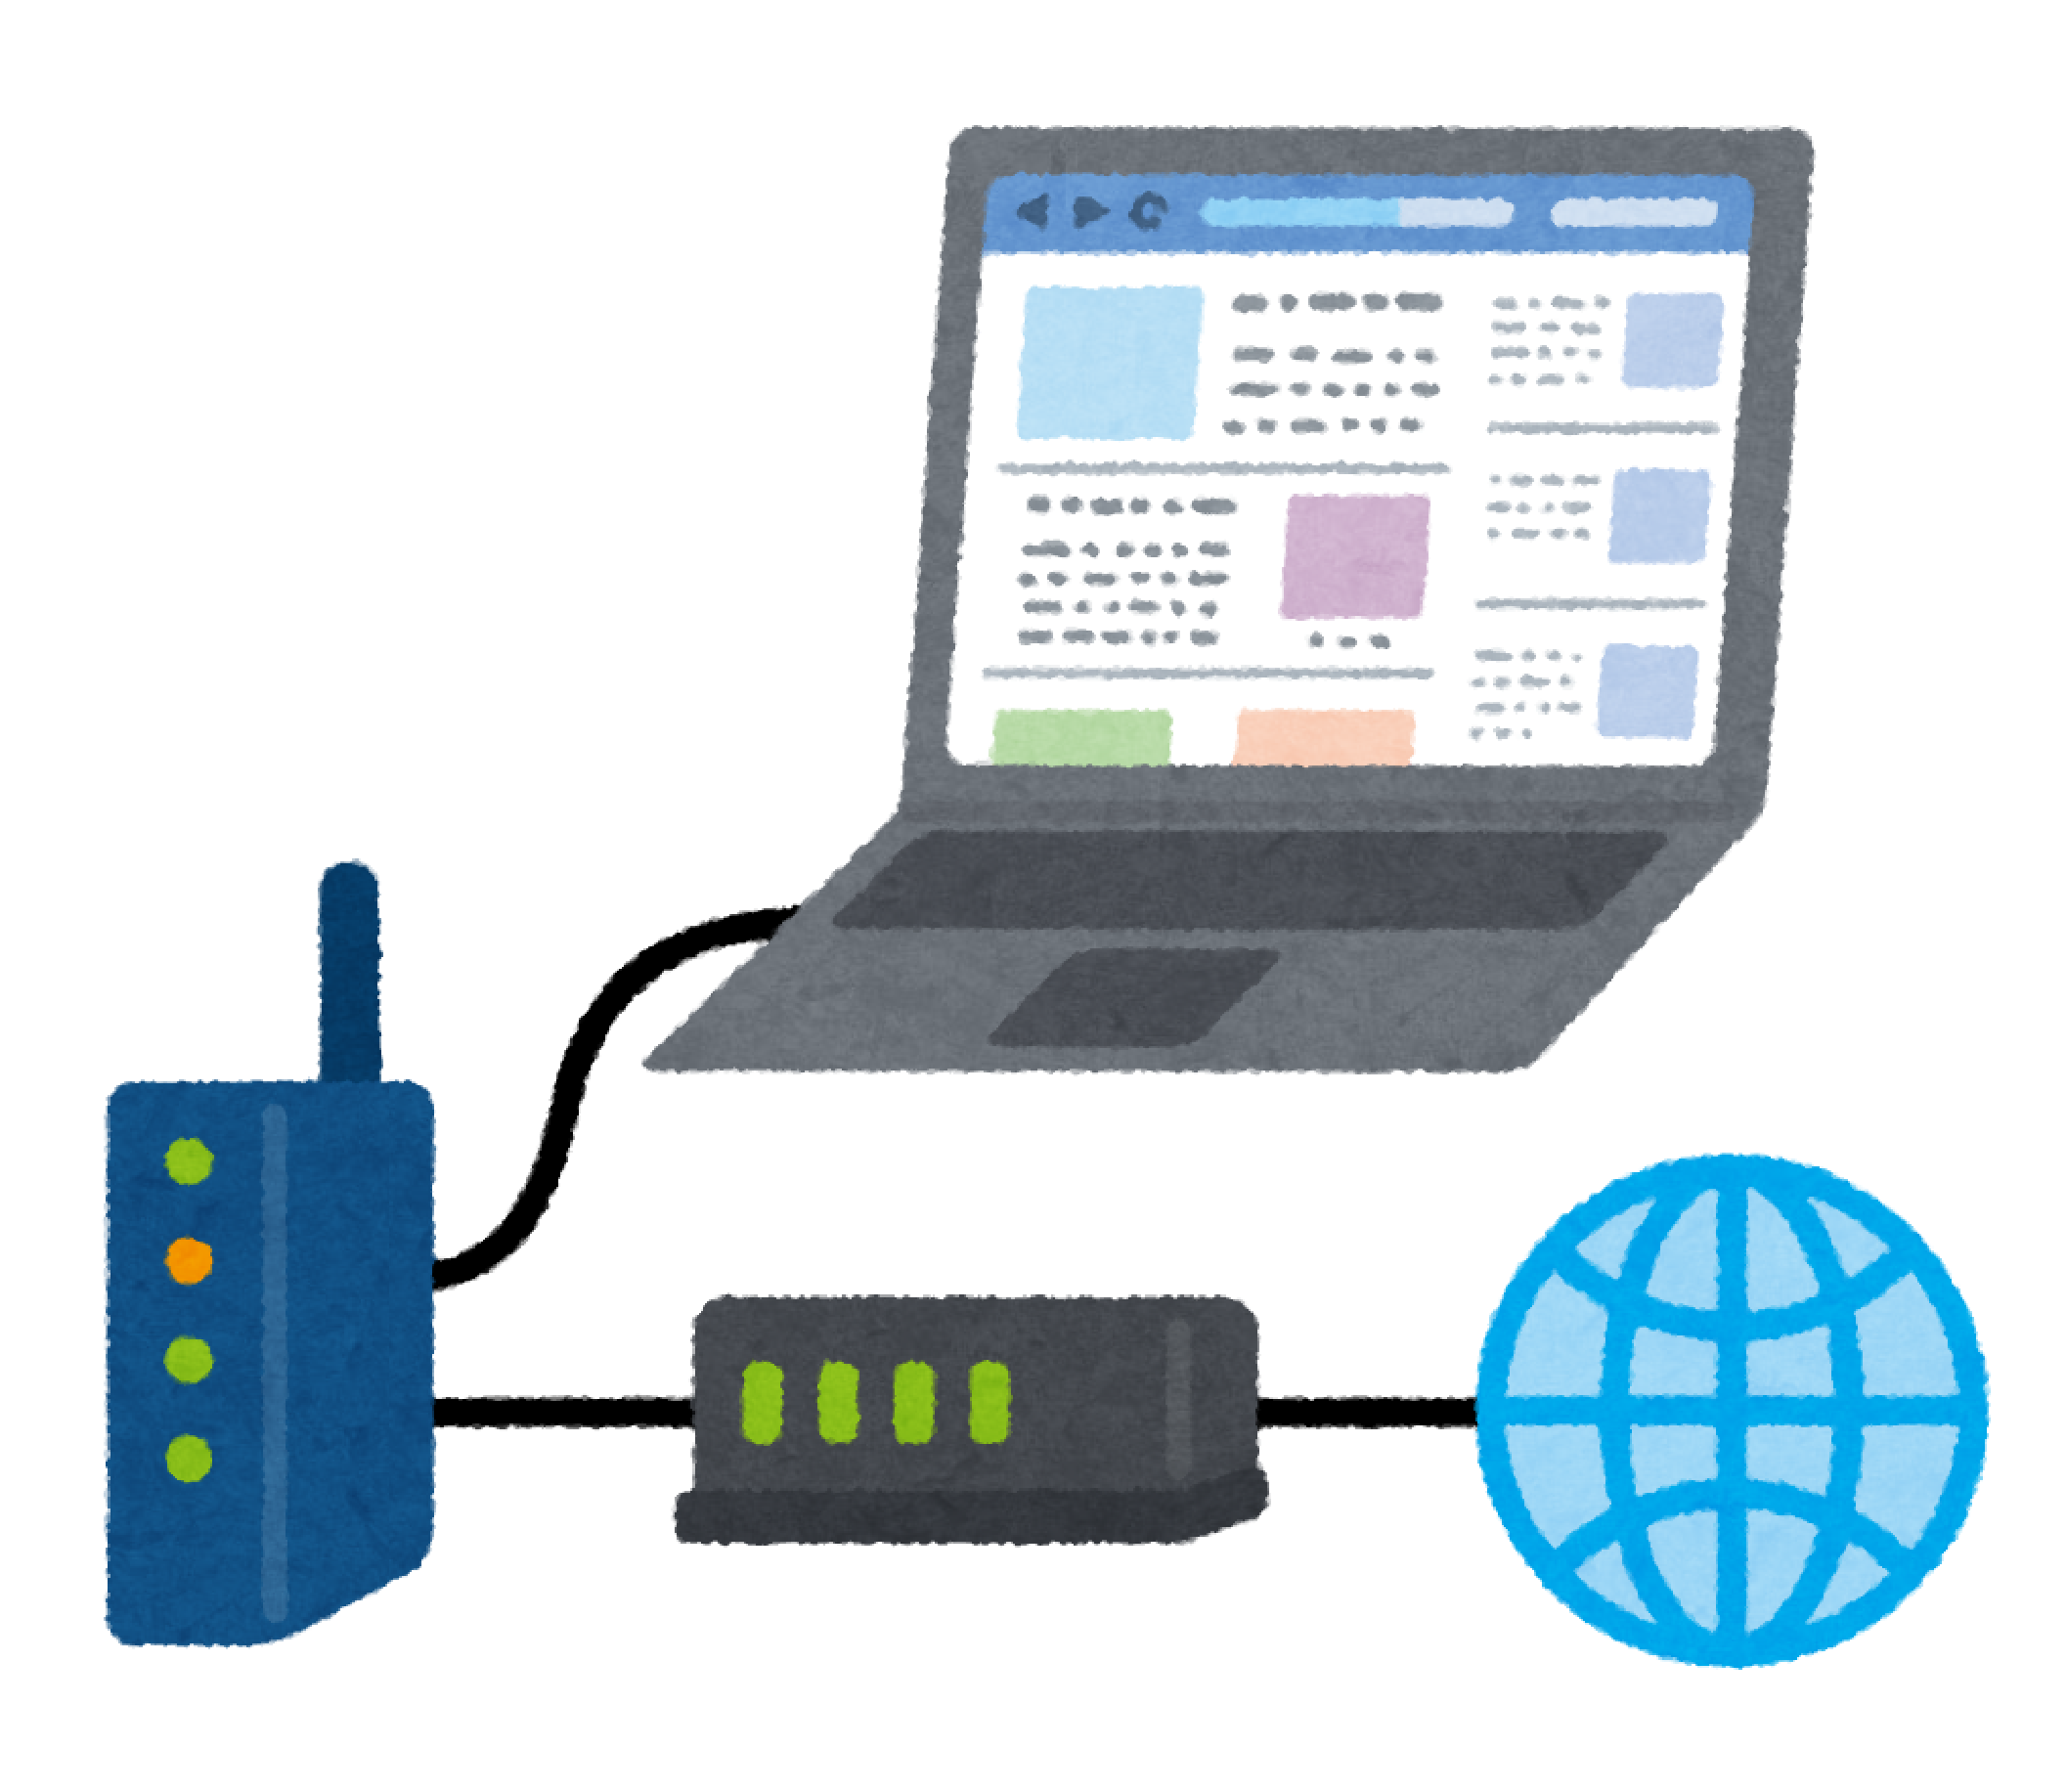
\includegraphics[width=7.0cm]{./pic/internet_computer_wired.png.pdf}
				\caption{1枚目 \label{fig:no1}}
				\end{minipage}
				\begin{minipage}[c]{0.5\hsize}
				\centering
				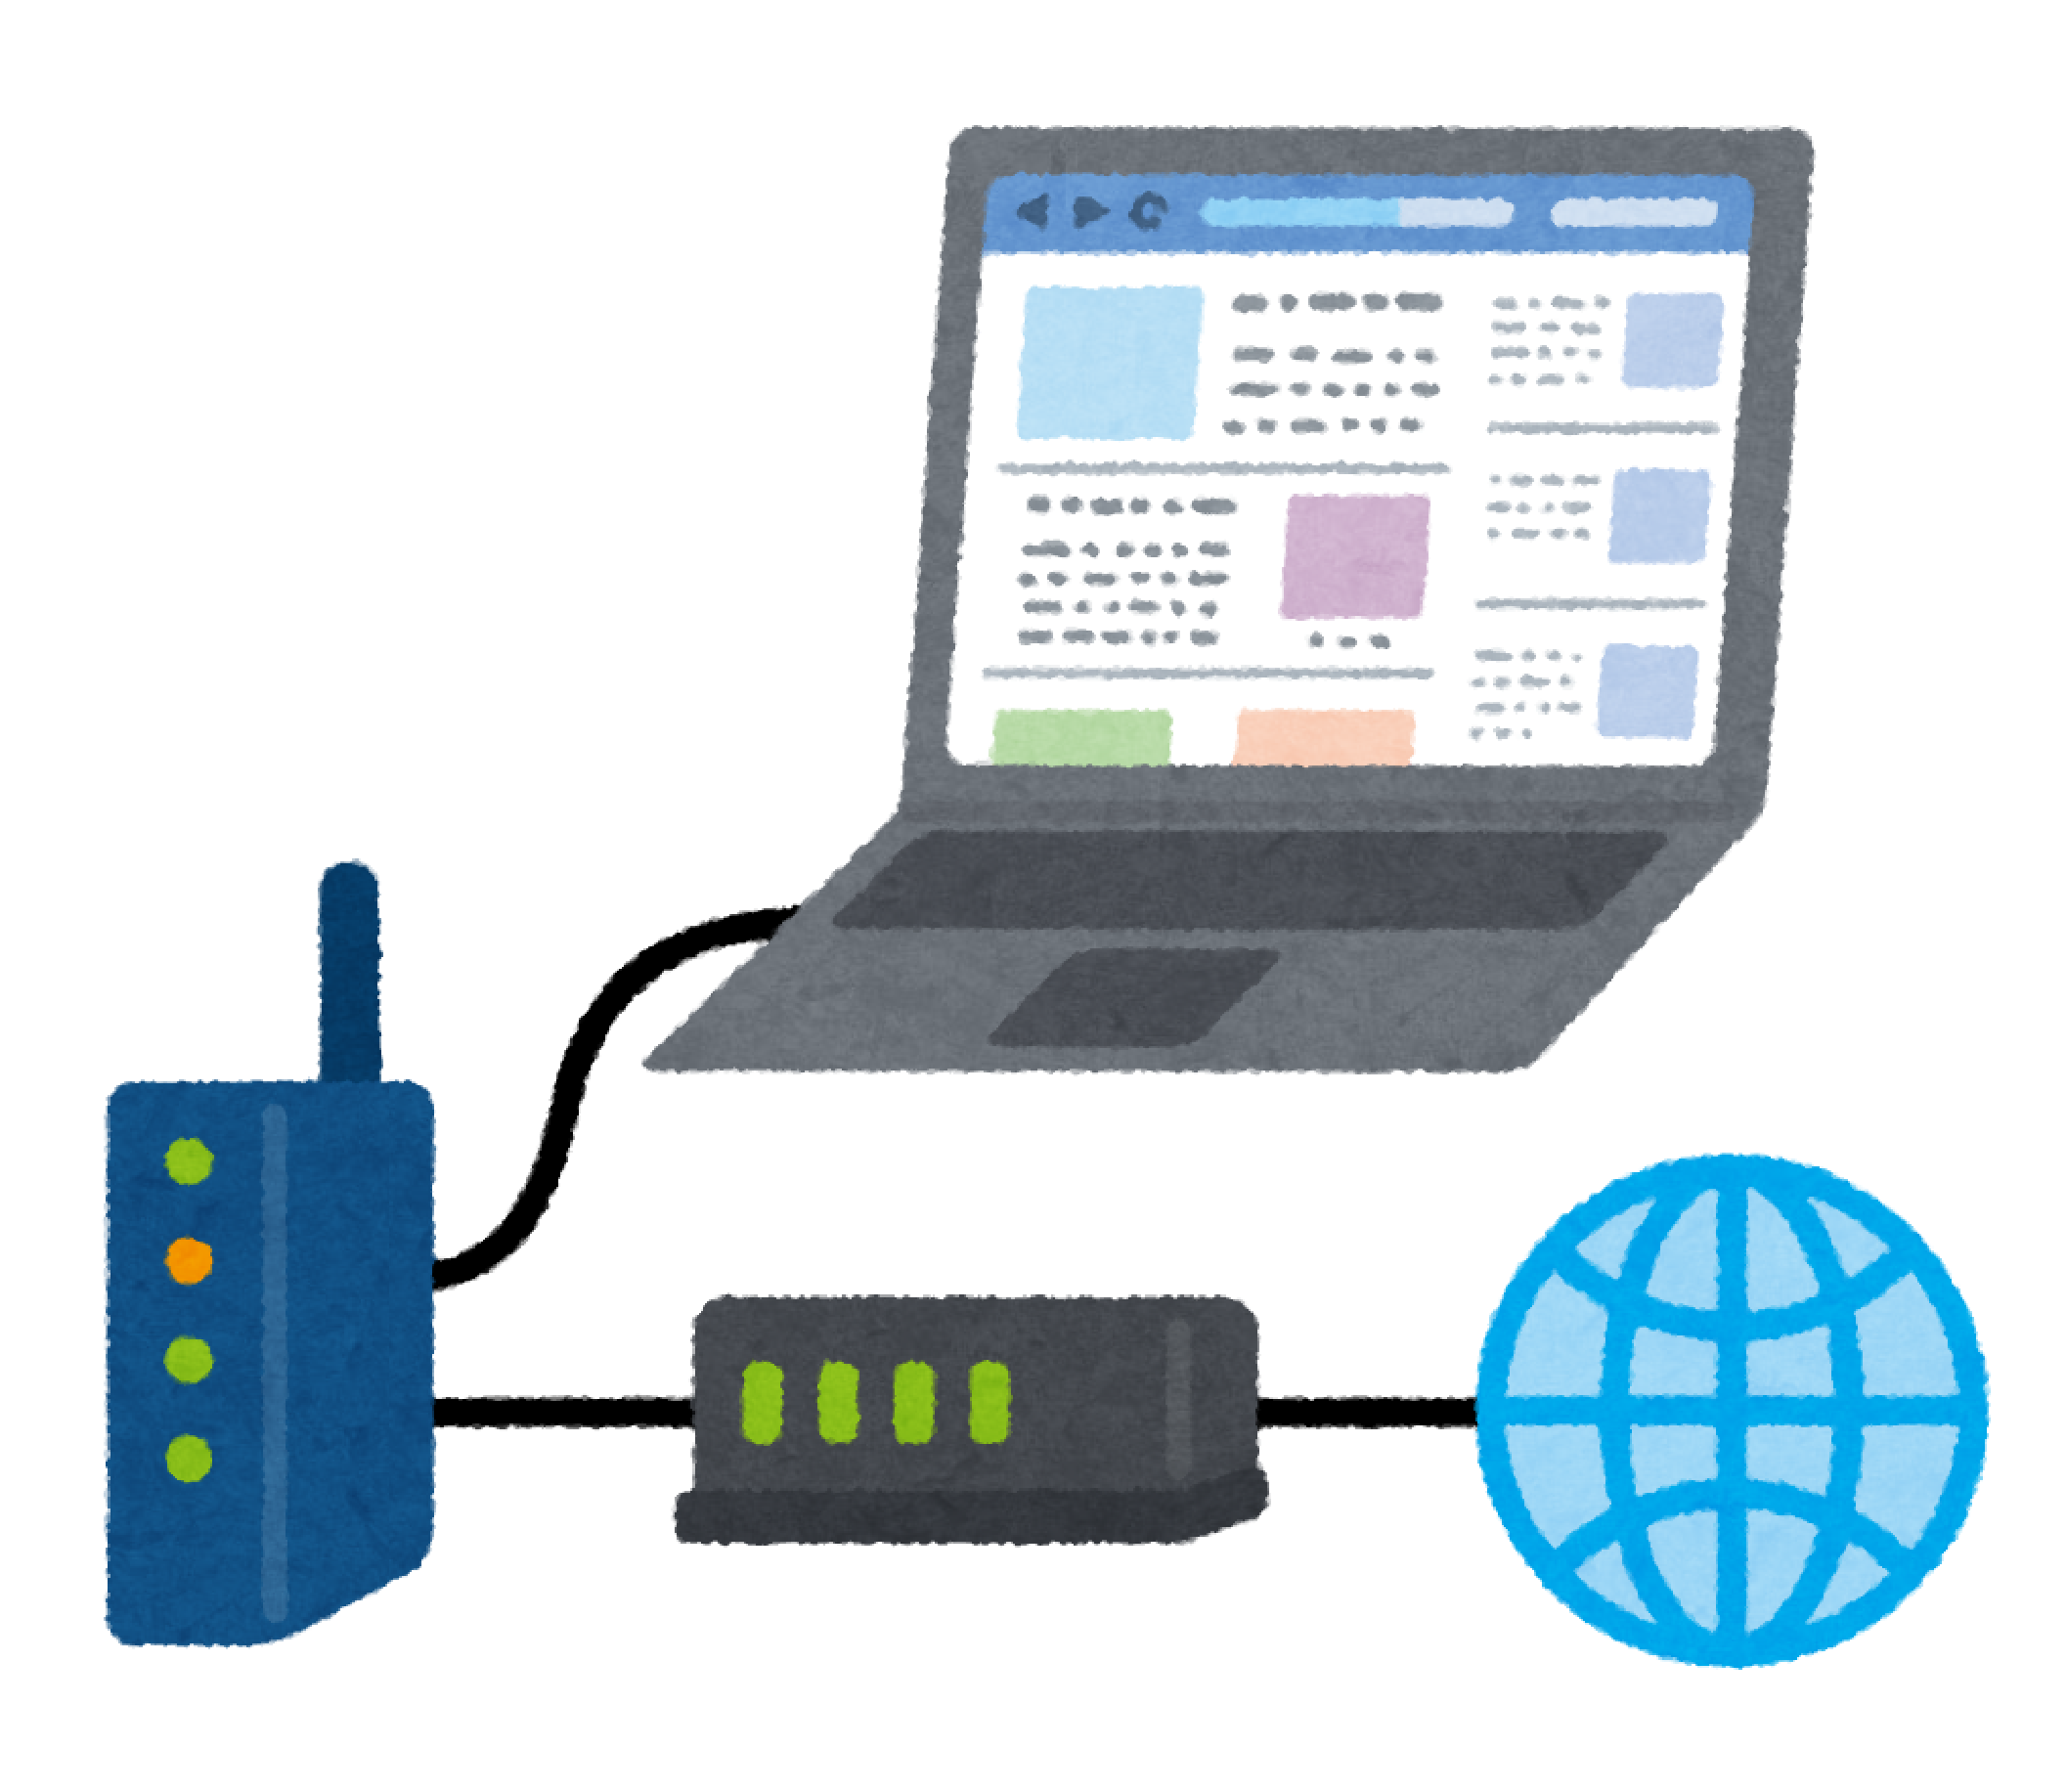
\includegraphics[width=7.0cm]{./pic/internet_computer_wired.png.pdf}
				\caption{2枚目 \label{fig:no2}}
				\end{minipage}
			\end{figure}
	\section{表の書き方編}
		\begin{table}[H]
			\centering
			\caption{サンプル表 \label{tab:sample}}
			\begin{tabular}{|c||c|c|c|}
				\hline  & 電流$[A]$ & 電圧$[V]$ & 時間$[s]$ \\ \hline \hline
				A & 1 & 10 & 0.01 \\ \hline
				B & 2 & 0.4 & 0.3 \\ \hline
				C & 3 & 1 & 0.6 \\ \hline
			\end{tabular}
		\end{table}
	\section{相互参照編}
		図\ref{fig:no1}は横並びの画像を指します。 \\
		式\ref{eq:univ_gravity}は万有引力の方程式を示しています。\\
		表\ref{tab:sample}はサンプルの表を示しています。 \\
		第\ref{math_mode}節では、数式モードの解説です。
	\section{参考文献編}
		参考文献\cite{my_blog}より、以上のことが証明される。
	\begin{thebibliography}{99}
		\bibitem{my_blog} だつかくあーてぃー, "LaTeX環境の構築", \url{https://datsuka-qwerty.hatenablog.com/entry/latex/linux_install}, アクセス・2023年7月22日
		\bibitem{hogehoge_book} hogehoe "ほげほげの本", はげはげ発行所, 発行・2023年7月22日
	\end{thebibliography}
\end{document}